\chapter{Results and Discussion}

\section{Exploratory Data Analysis}

\subsection{Weather}
\subsubsection{Seasonality}
\subsubsection{Trend of Disruptive Variables}


\subsection{Traffic}
\subsubsection{Seasonality}
\subsubsection{Previous Day}
\subsubsection{Previous Week}
\subsubsection{Connected Roads Segments}



\subsubsection{Rolling and Expanding Features}

The data only describes the traffic condition per timestep and the seasonality of traffic. Although traffic has pattern, there are instances when a certain disruption in traffic may cause congestion build up. Therefore, considering how the past traffic conditions may affect the current traffic condition can be considered as a factor for predicting traffic. Although the data from the previous timestep can be used as a reference in predicting the current traffic condition, the change in traffic in a 15-minute timeframe may not be significant. As seen in \figref{figure_autocorr_traffic_workingdays}, autocorrelation reveals that a traffic condition is highly likely to reoccur every 15 minutes with a correlation value of 0.9918. In other words, the traffic condition of the previous time step is highly likely to be the traffic condition of the current time step. However, this does not capture the effects of sudden outliers to the build up or decay of traffic. Thus, it does not fully describe how the past traffic conditions might affect the current traffic condition. 

\begin{figure}
  \centering
  \captionsetup{justification=centering}
  \scalebox{.80}{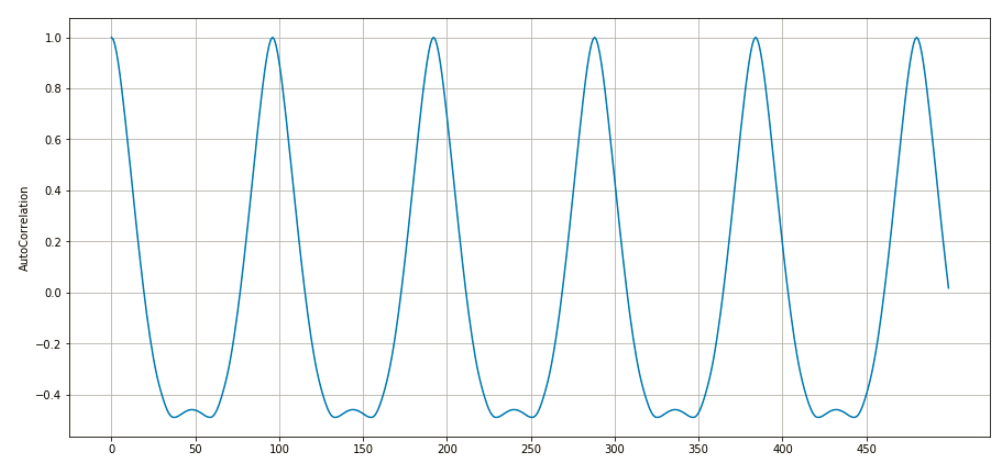
\includegraphics{autocorr_whyRE.PNG}}
  \caption{Autocorrelation of traffic for working days}
  \label{figure_autocorr_traffic_workingdays}
\end{figure}

Generating rolling and expanding features based on a specific window size gives a bigger look as to what the current traffic might be based from the previous traffic conditions. Rolling and expanding traffic features such as the mean, the minimum, and the maximum with window size  4, 8, 24, 48, and 96 were generated from the original traffic data. To summarize the possible effects of sudden changes in traffic, the mean of the past traffic conditions based on a window size was generated. Figure \ref{figure_stdev_traffic} shows the standard deviation values of traffic for every window size. Standard deviation shows the variability or the distance of the data from the mean. From this, it can be observed that there is a logarithmic pattern in the growth of the standard deviation as the window size increases. The low standard deviation of smaller window sizes signifies that there is only a little to no change in traffic condition within that time frame. Meanwhile, large window sizes like window 96 which yield a relatively larger standard deviation value of 0.03531 than of window 4, implies that the traffic conditions in a 1-day time frame are more varied or are more widely spread. With small window sizes, the values generated captures less of the trifle changes in traffic and gets more affected by outlier values which then results in a more generic information. However, as the window size increases, the effect of outlier values also get more neutralized because of the number of data considered, giving a broader summary of the past traffic. 

\begin{figure}
  \centering
  \captionsetup{justification=centering}
  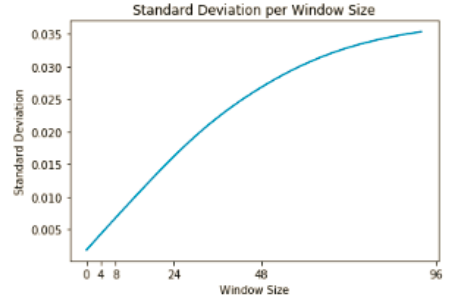
\includegraphics{stDev.PNG}
  \caption{Standard deviation per window size of northbound traffic in Bluementritt for wet season}
  \label{figure_stdev_traffic}
\end{figure}


Unlike the rolling mean, the expanding mean bases its computations on a growing window size and goes back to window size 1 when it reaches a specific maximum window size. This lessens the probability of the outliers getting majorly and consistently neutralized since it always goes back to the original traffic condition from the previous timestep. Thus, revealing less generalized details.

The minimum and maximum features, on the other hand, reveals the range of the dataset. Being sensitive to outliers, they provide outlier detection when compared to the average value of that specific set of data. A big difference between the values of the minimum and the maximum signifies a large progression in traffic condition. Although as the window size used gets bigger, it becomes harder to determine whether the sudden change in traffic condition occurred just a few timesteps before or if it is because of a farther instance which may have less to no effect to the current traffic condition. 

Figures \ref{fig:EspanaRE} and \ref{fig:RoxasRE} show the average correlation of northbound road segments of Espana and southbound road segments of Roxas Boulevard per window size in relation to traffic for both rolling and expanding windows. On average, the original traffic has a strong relationship with rolling features having small window size, specifically window 4 with a correlation value of 0.7501. It is noticeable, however, that the strength of the relationship dwindles down as the window size increases. This reveals that although having a bigger window size means being able to capture various changes in traffic condition, it does not give importance to the most recent traffic conditions. Big changes in traffic conditions that occurred way back and may not have any effect on the current traffic are being considered. Thus, causing its misalignment to the original data. 

In the case of expanding windows, the strength of the relationship to the original traffic also decreases as the window size increases, albeit not so much as the rolling mean do. Looking into both graphs, the strength of the relationship given by window 4 for both rolling and expanding is distinctly stronger compared to the ones with larger window size. This might be because as mentioned earlier, traffic does not usually change significantly within a small window. Furthermore, a smaller window size means that its frequency of reverting back to the original value, making its generated value more accurate. Meanwhile, the farther from the past that it considers, the less it captures changes in traffic. This is shown in Figures \ref{fig:bluementritt_rolling} and \ref{fig:bluementritt_expanding}, where rolling and expanding at window 96 generalizes the high condition intensities into information that is no longer close to reality. Furthermore, the plodding decrease of correlation strength in expanding features as compared to rolling features is caused by limiting the number of windows that the feature grows to and considers and the restarting of its window size. Not limiting the window size growth of expanding features would produce values that are very far away from reality because it would consider every data from the previous days. It would contain values that consider data that are not relevant in predicting the future traffic.



\begin{figure}
    \centering
      \captionsetup{justification=centering}
    \subfloat[EspanaRE]{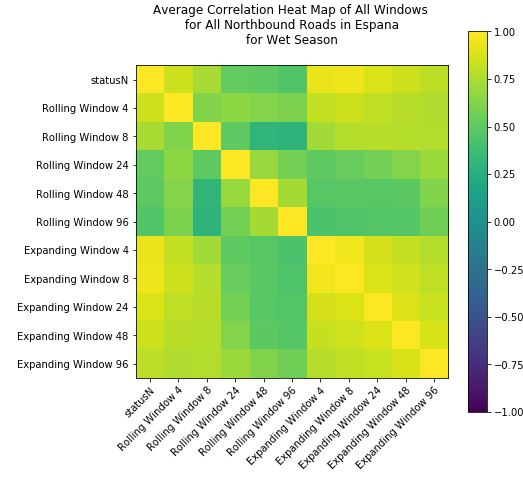
\includegraphics[width=0.5\textwidth]{figures/heatmap_espana.JPG}\label{fig:EspanaRE}}
    \hfill
    \subfloat[RoxasRE]{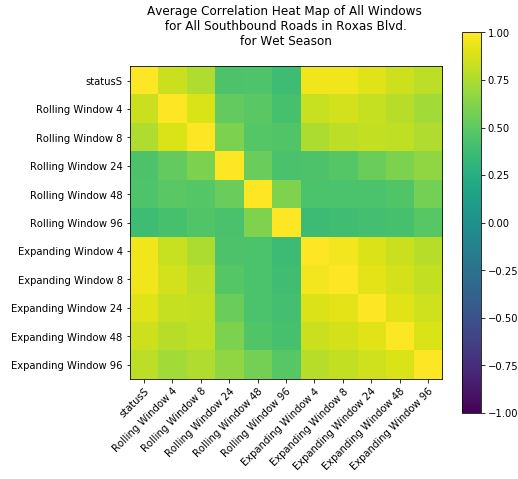
\includegraphics[width=0.5\textwidth]{figures/heatmap_roxas.JPG}\label{fig:RoxasRE}}
    \caption{Average Correlation of Rolling and Expanding Features for Espana and Roxas Blvd.}
\end{figure}

\begin{figure}
    \centering
      \captionsetup{justification=centering}
    \subfloat[Original vs. Rolling]{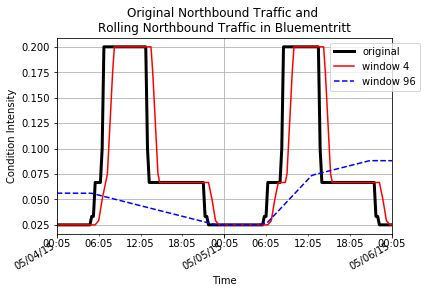
\includegraphics[width=0.5\textwidth]{bluementritt_rolling.png}\label{fig:bluementritt_rolling}}
    \hfill
    \subfloat[Original vs. Expanding]{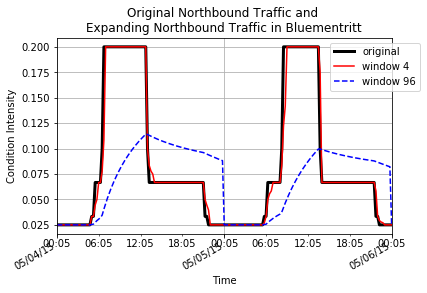
\includegraphics[width=0.5\textwidth]{bluementritt_expanding.png}\label{fig:bluementritt_expanding}}
    \caption{Comparison of Rolling and Expanding windows 4 and 96 to original Southbound traffic in Bluementritt}
\end{figure}


\subsection{Relationship of Weather to Traffic}
\subsubsection{Daytime and Nighttime}
\subsubsection{Time of Day}


\subsection{Effects of Weather to Traffic}
\subsubsection{Precipitation}
\subsubsection{Season by Precipitation Rate}
\subsubsection{Weather Disruption}



\section{Prediction Model Analysis}

\subsection{Traffic-Only Model}
\subsection{Weather-Only Model}
\subsection{Fusion Analysis}
\subsection{Sensitivity Analysis}